\documentclass{report}
\usepackage[english]{babel}
\usepackage{illcmolthesis}
\usepackage{microtype}
\usepackage{amsmath,amssymb}
\usepackage{amsthm}
\usepackage[round, authoryear]{natbib}
\usepackage[all]{xy}
\usepackage{array}
\usepackage{graphicx}
\usepackage{framed}
\usepackage{enumerate}
\usepackage{qtree}
\usepackage{mdframed}
\usepackage{tikz}
\usepackage{multirow}
\usepackage{pgfplots}
\pgfplotsset{compat = newest}
\usepackage{tikz-dependency}
\usetikzlibrary{matrix}
\usepackage{xfrac}
\usepackage{algorithmic}
\usepackage{pdfpages}
\usepackage{algorithm}
\usepackage{float}
\usepackage[OT2,T1]{fontenc}
\usepackage{hyperref}
%\usepackage[a4paper]{geometry}
\newcommand\textcyr[1]{{\fontencoding{OT2}\fontfamily{wncyr}\selectfont #1}}
\newcommand{\myparagraph}[1]{\paragraph{#1}\mbox{}\\}
\bibliographystyle{plainnat}
\renewcommand\topfraction{0.85}
\renewcommand\bottomfraction{0.85}
\renewcommand\textfraction{0.1}
\renewcommand\floatpagefraction{0.85}

%Define theorem style for definition and metric
\newtheoremstyle{break}  % follow `plain` defaults but change HEADSPACE.
  {\topsep}   % ABOVESPACE
  {15pt}   % BELOWSPACE
  {\itshape}  % BODYFONT
  {0pt}       % INDENT (empty value is the same as 0pt)
  {\bfseries} % HEADFONT
  {.}         % HEADPUNCT
  {\newline}  % HEADSPACE. `plain` default: {5pt plus 1pt minus 1pt}
  {}          % CUSTOM-HEAD-SPEC

\theoremstyle{break}
\newtheorem{metric}{Metric}
\newtheorem{notion}{Notion}
\newtheorem{definition}{Definition}
\def\citepos#1{\citeauthor{#1}'s (\citeyear{#1})}

%Define new float environment for tables that is boxed
\floatstyle{boxed}
\newfloat{tab}{tbp}{lop}
\floatname{tab}{Table}


\begin{document}

\chapter{Empirical Research on Transfer Models}

Chapter introduction, but an overall analysis of how well monolingual compositionality and bilingual compositionality actually match up ... 

we will focus on HATs
We will study the consitency of HATs and dependency grammars, and study the main causes of deviation of the translation structures from conventional linguistic syntax. We will present an easily accessible implementation, that is reusable for various purposes and is thus suitable for further investigation by others. In this chapter, we motivate and explain the procedures that were used, and .... We will start by discussing our translation structures... on a more intuitive level.

\section{Bilingual Compositionality}

Recall: translations structures
In this thesis, we will consider a subset of all alignment trees, that was already mentioned in the previous chapter: the HATs \citep{simaan2013hats}. A HAT is characterized by the fact that it is maximal, i.e., every node has its minimal branching factor.\footnote{Say something about node operators and skeleton} This means that every non-terminal node is expanded into a minimum number of children, but also that phrases are used \textit{only} when they are needed to account for the translation phenomena. An example that illustrates this is depicted in Figure \ref{fig:treephrase}.

\begin{figure}
\centering
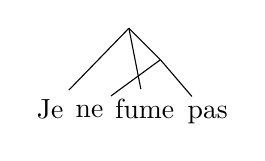
\begin{tikzpicture}

\node (je) at (0,0.07) {Je};
\node (ne) at (0.5,0.04) {ne};
\node (fume) at (1.2,0.08) {fume};
\node (pas) at (2,0) {pas};

\coordinate (nepas) at (1.4,0.7);
\coordinate (jefume) at (0.6,0.7);
\coordinate (all) at (1.0,1.1);

\draw (nepas) -- (ne);
\draw (nepas) -- (pas);
\draw (je) -- (all);
\draw (fume) -- (all);
\draw (all) -- (nepas);

\end{tikzpicture}
\caption{Describe how a phrase-based translation system would consider `ne fume pas' als een phrase pair, and the underlying structure would be gone, while the HAT preserves the internal structure}\label{fig:treephrase}
\end{figure}


\subsection{Motivation}

There is a computational advantage to considering only minimally branching trees. Not only does it significantly reduce the space of trees to be considered (in case of the previous dog example, there are 5 trees instead of 44), it also simplifies parsing, as the lower-rank rules that can be extracted from minimally branching trees can be more efficiently treated by a parsing algorithms. Such considerations are very important when designing an MT model. Although it is even for an empirical analysis that the computational requirements match the reality, one might doubt whether restricting the set of trees to consider is theoretically justifiable. In the following paragraphs we will argue it is.

First of all, considering only maximally branching trees secures that the system we are studying is in fact compositional. The set of all compositional translation trees contains many flat trees, that can strictly speaking be seen as compositional (as compositionality is highly underspecified in this respect), but do not capture the recursive and systematic nature of language. A compositional system containing a separate rule for almost every sentence that specifies how the meaning can be derived from \textit{all of its words} does certainly not correspond with human intuitions about compositionality, not to mention the fact that such a grammar should be infinite to cover the entire language. Considering only minimally branching trees solves this problem.

Secondly, considering only expansions that are maximally compositional maximises the chanse that generalisation to new data is possible: a rule that specifies how a type of argument can be combined with a type of predicate is more useful than a rule specifying how the argument `I' can be combined with the predicate `like'. Minimum depth expansions are more probable to be applicable in new situations.

A special case that ties together the previous two arguments occurs with the treatment of phrasal translations. As the rest of the tree, sequences of words will be translated as a whole only if they do not have a deeper structure according to the translation data. In many phrase-based translation systems, including the successful hierarchical phrase based translation, the underlying system of sequences that are translated phrasally gets lost in the process, whereby the system misses an opportunity to detect a pattern. Figure \ref{fig:treephrase} illustrates the advantage of this property.

Of course, there are some cases in which assuming \textit{maximal} compositionality is a bit strict, and not consistent with what is actually going on. We will present solutions for these cases later.

\subsection{Intuition}

In words, the set of structures considered in this thesis can be characterised by the following properties:
\begin{enumerate}
\item The structures are projective trees.
\item The non-terminal nodes in the tree correspond to subsequences that were possible parts in the translation, while sibling terminal nodes toghether constitute a translation admissible part, herewith respecting the strategy of compositional translation.
\item Nodes can have both non-terminal nodes and terminal children.
\item All nodes of the tree have a minimal branching factor.
\end{enumerate}

\noindent The set of structures considered is thus associated with a synchronous context-free grammar, in which expansion into the most general non-terminals is preferred over expansions into words, and phrasal translations are used only when necessary. This captures the intuition that even in complicated cases like syntactic divergence, the parts constituting the most important elements of the sentence are grossly the same, and the difference in syntactic structure is reflected only in a few words. We will provide some examples to elucidate this.

\begin{figure}[!ht]
\centering
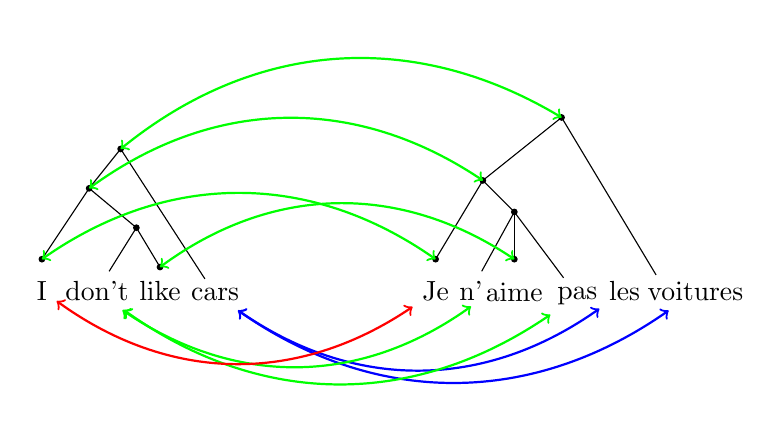
\begin{tikzpicture}
\draw node (I) at (0,0) {I};
\draw node (dont) at (0.7,0) {don't};
\draw node (like) at (1.5,0) {like};
\draw node (cars) at (2.2,-0.05) {cars};

\draw node (Je) at (5.0,0) {Je};
\draw node (n) at (5.45,0) {n'};
\draw node (aime) at (6.0,-0.02) {aime};
\draw node (pas) at (6.8,-0.07) {pas};
\draw node (les) at (7.4,0) {les};
\draw node (voitures) at (8.3,-0.01) {voitures};

\coordinate (Je_) at (5.0,0.4);
\coordinate (like_) at (1.5,0.3);
\coordinate (I_) at (0,0.4);
\coordinate (aime_) at (6.0,0.4);
\coordinate (naimepas) at (6.0,1);
\coordinate (dontlike) at (1.2,0.8);
\coordinate (Idontlike) at (0.6,1.3);
\coordinate (Jenaimepas) at (5.6,1.4);
\coordinate (lesvoitures) at (7.8,0.2);
\coordinate (all) at (1,1.8);
\coordinate (tout) at (6.6,2.2);
\coordinate (n_) at (5.45,-0.2);

\foreach \coordinate in {dontlike, like_, I_, Je_, aime_, Idontlike, all, tout, Jenaimepas, naimepas}
	\filldraw (\coordinate) circle (0.035);

\foreach \from/\to in {naimepas/aime_, naimepas/n, naimepas/pas, dontlike/like_, dontlike/dont, Idontlike/I_, Idontlike/dontlike, all/Idontlike, all/cars, Jenaimepas/Je_, Jenaimepas/naimepas, tout/Jenaimepas, tout/lesvoitures}
	\draw (\from) -- (\to);

\foreach \from/\to in {cars/voitures, cars/les}
	\draw[<->, bend left = -35, thick, blue] (\from) to (\to);

\foreach \from/\to in {dont/n_, dont/pas, tout/all, Jenaimepas/Idontlike, aime_/like_, Je_/I_}
	\draw[<->, bend left = -35, thick, green] (\from) to (\to);

\draw[<->, bend left = -35, thick, red] (I) to (Je);

\end{tikzpicture}
\caption{Translation of negation, French-English}\label{fig:nepas}
\end{figure} 


A famous example that is often taken as troublesome in MT (refs?) is the translation of (English) negation in the non-contiguous French `ne ... pas'. Figure \ref{fig:nepas} shows a compositional translation tree that accounts for such a translation in the system sketched in this thesis. The translation tree shows that `I dont like' is the translation of `Je n'aime pas', but also contains the information that `don't' is phrasally translated as `ne ... pas'. Removing the negation in the English sentence results in the grammatical English sentence `I like cars', removing its translation equivalent in the France sentence in its (almost) grammatical `Je aime les voitures'. 

An example containing syntactic divergence in translation between Russian and English is depicted in Figure \ref{fig:russian}. In Russian, `X has Y` is (communistically) translated as `with X is Y', the object in English is thus the subject in Russian. Figure \ref{fig:russian} shows how this is dealt with in a translation structure. Note that although this translation tree is easily extendible to longer sentences with the same construction. By expanding the non-terminal nodes it can also capture sentences like `the girl with the long blond hair has a very old car with broken windows'.

\begin{figure}[!ht]
\centering
\begin{tikzpicture}

\draw node (the) at (0,0.02) {The};
\draw node (girl) at (0.75,0) {girl};
\draw node (has) at (1.4,0.04) {has};
\draw node (a) at (1.9,0) {a};
\draw node (car) at (2.4,0) {car};
\draw node (y) at (4,0) {\textcyr{u}};
\draw node (girlr) at (4.9,-0.02) {\textcyr{devuxka}};
\draw node (is) at (6.1,0.02) {\textcyr{est\char126}};
\draw node (carr) at (7.5,0.04) {\textcyr{avtomobil}};

\coordinate (thegirl) at (0.4,0.6);
\coordinate (acar) at (2.1,0.6);
\coordinate (thegirlhas) at (0.8,1);
\coordinate (all) at (1.4,1.5);
\coordinate (carr_) at (7.5, 0.3);
\coordinate (girlr_) at (4.9,0.3);
\coordinate (girlhas) at (4.9,0.8);
\coordinate (allr) at (5.9, 1.2);


\foreach \coordinate in {thegirl, acar, thegirlhas,all,carr_, girlr_, girlhas, allr}
	\filldraw (\coordinate) circle (0.035);

\foreach \from/\to in {thegirl/girl, thegirl/the, acar/a, acar/car, thegirlhas/thegirl, thegirlhas/has, all/thegirlhas, all/acar, girlhas/girlr_, girlhas/y, girlhas/is, allr/girlhas, allr/carr_}
	\draw (\from) -- (\to);

\foreach \from/\to in {the/girlr, girl/girlr}
	\draw[<->, bend left = -35, thick, blue] (\from) to (\to);

\foreach \from/\to in {has/y, has/is, allr/all, girlhas/thegirlhas, carr_/acar, girlr_/thegirl}
	\draw[<->, bend left = -35, thick, green] (\from) to (\to);

\foreach \from/\to in {a/carr, car/carr}
	\draw[<->, bend left = -35, thick, red] (\from) to (\to);


\end{tikzpicture}
\caption{Translation of possession, Russian-English}\label{fig:russian}
\end{figure}

\subsection{Representation and Generation}

To study HATs, we need to be able to generate the set of HATs for every sentence. As generating and storing all trees separately would be both time and space consuming, and would impede a flexible search through them, hence a suitable representation of the set of HATs is required. In this thesis, we will represent the set of HATs for a sentence implicitly by a context-free grammar, whose node labels correspond to the spans the respective node covers (anders). An example can be found in Figure \ref{fig:grammar}

\begin{figure}[!ht]\begin{framed}
\small{
\begin{tabular}{llllll}
(0-6] $\rightarrow$ (0-1]  (1-6] && (4-6] $\rightarrow$ (4-5]  (5-6] && (0-1] $\rightarrow$ My\\
(0-6] $\rightarrow$ (0-2]  (2-6] && (0-4] $\rightarrow$ (0-1]  (1-4] && (1-2] $\rightarrow$ dog\\
(0-6] $\rightarrow$ (0-4]  (4-6] && (0-4] $\rightarrow$ (0-2]  (2-4] && (2-3] $\rightarrow$ also\\
(1-6] $\rightarrow$ (1-4]  (4-6] && (1-4] $\rightarrow$ (1-2]  (2-4] && (4-5] $\rightarrow$ eating\\
(1-6] $\rightarrow$ (1-2]  (2-6] && (0-2] $\rightarrow$ (0-1]  (1-2] && (5-6] $\rightarrow$ sausages\\
(2-6] $\rightarrow$ (2-4]  (4-6] && (2-4] $\rightarrow$ (2-3] likes\\
\end{tabular}
\caption{The grammar generating the translation tree forest for the sentence
`My dog also likes eating sausages', with set-permutation $\langle _0\{0\}_1,~ _1\{1\}_2,~ _2\{3\}_3,~ _3\{2,4\}_4, ~_4\{6\}_5,~ _5\{5\}_6\rangle$ would be (the subscripts indicating the span annotation, which is left exclusive and right inclusive)}\label{fig:grammar}
}
\end{framed}
\end{figure}

The allowed expansions were found with an algorithm similar to \citepos{dijkstra1959note} shortest path algorithm (Algorithm \ref{alg:shortest paths}), that was adapted to be more efficient given the extra knowledge of the alignment graph.

\begin{algorithm}[!ht]
\caption{Shortest Paths}\label{alg:shortest paths}
\begin{algorithmic}
\STATE \textbf{Input:} A graph $G = (V,E)$ describing an alignment and two vertices $i$ and $j$ for which $(i,j)\in E$ is true.
\STATE \textbf{Output:} All non-trivial shortest paths from $i$ to $j$
\STATE \textit{\#Initialization}
\STATE visited = $\emptyset$, depth = $0$, paths = $\{j\}$
\STATE $\forall n\in\mathbb{N}:$ reachable(n) = $\emptyset$; reachable($0$) = $\{j\}$
\STATE depth\_finished = False
\STATE \textit{\# Start backwards search through graph}
\WHILE{not depth\_finished or $i\notin$ visited}
	\WHILE{reachable(depth) $\neq\emptyset$}
		\STATE depth\_finished $\leftarrow$ False
		\STATE current\_node $\leftarrow N$ an arbitrary element $v$ from reachable(depth)
		\STATE reachable(depth) $\leftarrow$ reachable(depth) $-$ $\{$current\_node$\}$
		\FOR{ ($l$,current\_node) $\in E$}
			\IF{$l\notin $visited $\cup$ reachable(depth) \AND depth $\neq 0$}
				\STATE reachable(depth+1) $\leftarrow$ reachable(depth+1) $\cup$ $\{l\}$
				\FOR{path (current\_node,\ldots, $j) \in$ paths}
					\STATE path $\leftarrow$ ($l$,current\_node,\ldots, $j)$
				\ENDFOR
			\ENDIF
		\STATE visited $\leftarrow$ visited $\cup$ $\{l\}$
		\ENDFOR
	\STATE depth\_finished $\leftarrow$ True
	\STATE depth $\leftarrow$ depth+1
	\ENDWHILE
\ENDWHILE
\STATE \textbf{Return} paths
\end{algorithmic}
\end{algorithm}


\section{Monolingual Compositionality}

Intro, we use dependency parses blablabla. In the previous chapter, we have defined dependency grammars and parses in a very general fashion. We have already defined dependency parses in the previous chapter, and will not do that again.



Following common practice when using dependency structures, in this thesis it is assumed the dependency structure satisfies the following two conditions:\begin{enumerate}
\item When seen as a relation, $D$ constitutes a single-headed a-cyclic graph in which the words in $s$ are the nodes. (tree-constraint)
\item When the words are placed in the original order, the branches of the dependendency tree do not cross. (projectivity)
\end{enumerate}


\subsection{Representation}

We will represent a dependency parse as a set of relations, as is expressed in the following definition:\footnote{Note that this definition is different from the def....}

\begin{definition}[Dependency structure]
A dependency structure of a sentence $s = w_0\cdots w_n$ is a set of dependencies $D = \{ (i,j) |$ there is a dependency arrow from word $w_i$ to word $w_j \}$. 
\end{definition}

Formally, dependency grammars are not interpreted as compositional grammars, as they do not postulate the existence of non-terminal syntactic categories and therefore do not explicitly specify how a sentence was bult up from its parts. However, dependency graphs do give rise to an hierarchical structure, that specifies from which smaller parts the sentence was composed. For instance, the dependency graph depicted in Figure \ref{fig:deptree1} tells us that `likes' is the head word of the sentence, and that the sentence is composed of 4 parts: the head `likes', its modifier `also', its noun subject whose head is `dog' and the open clausal complement whose head is `eating'. The complement and subject are further divisible in `My' and `dog', and `eating' and `sausage', respectively. As the tree is projective, all parts are continuous. Also the graph in Figure \ref{fig:depgraph} prescribes an hierarchical structure: it is composed of the subject `I', the headword `know', and the phrase headed by `liet', that is in its turn built up from its head `liet', `dat', `hij' and the discontinous phrase `me winnen'. Such an hierarchical structure can not be captured by a phrase structure grammar.



\begin{figure}[!h]\label{fig:deptree1}
\centering
\begin{dependency}[theme=simple]%[hide label]
\begin{deptext}[column sep=.5cm, row sep=.1ex]
%PRP\$ \& NN \& RB \&[.5cm] VBZ \& VBG \& NN \\
My \& dog \& also \& likes \& eating \& sausage \\
\end{deptext}
\deproot{4}{}
\depedge{2}{1}{poss}
\depedge{4}{2}{nsubj}
\depedge{4}{3}{xvmod}
\depedge{4}{5}{xcomp}
\depedge{5}{6}{dobj}
\end{dependency}
\caption{Stanford Dependency Tree}
\end{figure}

\subsection{Generation}

To assign dependency structures to sentences, we used the Stanford Dependency Parser, that can be downloaded from their website, as well as used online  \citep{de2006generating}. The parser provides 5 variants of a typed dependency representation, of which the most basic one corresponds to the earlier imposed conditions on dependency structures. A picture of a dependency parse that was  generated by the parser is depicted in Figure \ref{fig:deptree1}. The Stanford Dependency parser does not include relations between words and punctuation, which is suboptimal, as they occur a lot in blabla. We will later explain how the problems arising from this fact were dealt with.

\section{Combining HATs and Dependency Parses}

%zeg anders, meer belangrijk, meer gerelateerd aan het grote plaatje: de vraag in deze thesis
To combine dependency parses and translation structures, means need to be find to quantify consistency and similarity between them. We have arrived at the situation depicted in Figure \ref{fig:depshats}.

\begin{figure}[!ht]
\centering
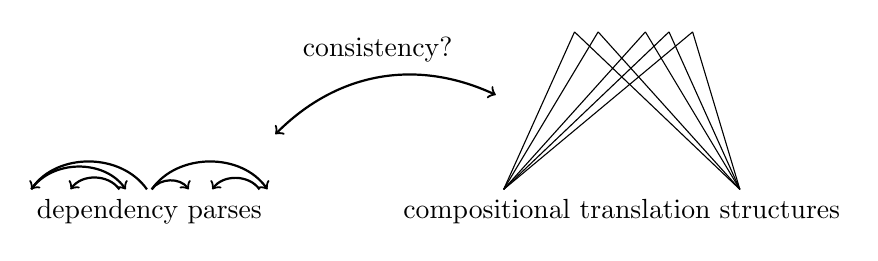
\begin{tikzpicture}

\coordinate (ss) at (1.5,0);
\node [below] at (ss) {dependency parses};

\draw[->,bend right = 55,thick] (1.47,0) to (0,0);
\draw[->,bend left = 55, thick] (1.53,0) to (3,0);
\draw[->,bend left = 55, thick] (0.0,0) to (1.2,0);
\draw[->,bend right = 55,thick] (1.12,0) to (0.5,0);
\draw[->,bend left = 55, thick] (1.53,0) to (2.0,0);
\draw[->,bend right = 55,thick] (2.9,0) to (2.3,0);

\coordinate (ts) at (7.5,0);
\node [below] at (ts) {compositional translation structures};

%\draw (6,0) -- (0.6,2) (9,0) -- (6.6,2);
\draw (6,0) -- (6.9,2) (9,0) -- (6.9,2);
\draw (6,0) -- (7.2,2) (9,0) -- (7.2,2);
%\draw (6,0) -- (7.5,2) (9,0) -- (7.5,2);
\draw (6,0) -- (7.8,2) (9,0) -- (7.8,2);
\draw (6,0) -- (8.1,2) (9,0) -- (8.1,2);
\draw (6,0) -- (8.4,2) (9,0) -- (8.4,2);

\coordinate (startarrow) at (3.1,0.7);
\coordinate (endarrow) at (5.9,1.2);
\node (t) at (4.4,1.5) [above]{consistency?};

\draw[<->,bend left =35, thick] (startarrow) to (endarrow);

\end{tikzpicture}
\caption{New situations: finding consistency between dependency parses and compositional translation structures}\label{fig:depshats}
\end{figure}

Explain how it is not immediately clear how dependency parses and translation structures: when they are the same they should get an optimal score, and when they are really different not, even if some parts are maybe still the same

explain different kinds of similarity

\subsection{Definitions of Consistency}

\subsection{Based on Labels}

Explain based on labels, F-score like, explain why not suitable (give example preferably!)

\subsection{Based on Relations}

Still several ways this can be done. Definitions based on whether a relation is respected by the HAT

\subsection{Scoring Trees}

\section{Implementation}

Say something about the fact that the real implementation is documented and available ... give some details as to how it was found.


\bibliography{thesisDH}
\end{document}